\documentclass[10pt,a4paper]{article}
\usepackage{fontspec}
\usepackage[spanish,es-noshorthands]{babel}
\usepackage[margin=2.2cm]{geometry}
\usepackage{amsmath,amssymb,booktabs,graphicx,siunitx,xcolor,caption,array,microtype}
\usepackage{xurl}
\usepackage{adjustbox}
\usepackage[colorlinks,linkcolor=teal,citecolor=teal,urlcolor=teal,pdftitle={Viviendas y población expuestas al aluvión de San Carlos de Apoquindo},pdfauthor={Lester Wood},pdflang={es-CL}]{hyperref}
\usepackage[natbibapa]{apacite}
\renewcommand{\doiprefix}{https://doi.org/\ignorespaces}
\AtBeginDocument{\renewcommand{\BRetrievedFrom}{}}
\sisetup{output-decimal-marker={,},group-separator={.},group-minimum-digits=4,group-digits=integer}
\captionsetup{font=small,labelfont=bf}
\graphicspath{{figs/}}

\title{Viviendas y población expuestas al aluvión de San Carlos de Apoquindo\\(Las Condes, 8 de octubre de 2026): estimación a partir de la\\propagación simulada, datos censales y curvas de vulnerabilidad}
\author{Lester Wood\thanks{Estudio independiente; documento derivado de \citet{wood2026}. Contenido bajo licencia CC BY-NC-SA 4.0. Condiciones de uso: \url{https://aluvion.hirely.cl/terminos.html}.}}
\date{Versión preliminar del 11 de octubre de 2026 (propagación de la primera generación)}

\begin{document}
\maketitle

\begin{abstract}
\noindent\textbf{Alcance.} Subestudio independiente, basado exclusivamente en datos públicos; sus resultados son calculados bajo supuestos, requieren validación científica independiente, no evalúan obras reales ni atribuyen responsabilidades. Usa las huellas de propagación de la primera generación del modelo (terreno con 1.103 edificios, 9--10 de octubre de 2026) y se actualizará con la versión con la ciudad completa.\par\medskip\noindent Se estimó la exposición potencial de edificios, viviendas y población censal a las huellas de propagación simuladas del aluvión de San Carlos de Apoquindo, y el daño esperado en los edificios. Para ello se cruzaron las manchas de propagación simuladas en el estudio principal con 42.018 huellas de edificios y con las 1.221 manzanas del Censo 2017 del área. El procedimiento de cruce territorial reproduce el de Hirely Broker, producto propio del autor. Las viviendas se asignaron por dos métodos, ponderación areal por manzana y asignación dasimétrica por huella de edificio, y el daño se estimó con dos curvas empíricas de vulnerabilidad para flujos de detritos. En el escenario que mejor reproduce el recorrido observado, el área con más de \SI{5}{cm} de barro contiene entre 2.360 y 2.950 viviendas según el método, y entre 2.060 y 3.240 en el análisis de sensibilidad; el balance preliminar de Senapred informó 2.361 viviendas afectadas. Entre 61 y 80 viviendas pertenecen a edificios con un grado de pérdida esperado de al menos 0,2, frente a 75 con daño mayor según Senapred y 55 inhabitables según el municipio. La longitud de calles con barro, \SI{15,3}{km}, es comparable con los \SI{15}{km} de avenidas dañadas que informó el municipio. Las cifras oficiales no se usaron para calibrar el modelo de propagación, pero su comparación con los resultados de exposición se hizo conociéndolas. Los resultados heredan la incertidumbre del modelo de propagación ---aún en fase de cribado--- y se recalcularán con el modelo definitivo.
\end{abstract}

\section{Introducción y planteamiento del problema}
La reconstrucción numérica del aluvión del 8 de octubre de 2026 \citep{wood2026} estima por dónde corrió el barro y con qué espesor y velocidad. Para la respuesta y la recuperación, sin embargo, la pregunta operativa es otra: cuántas viviendas y personas quedaron expuestas, con qué intensidad y cuántas viviendas sufrieron daño importante. Al día siguiente del evento, las cifras públicas eran balances preliminares levantados en terreno \citep{senapred2026latribuna,cnn2026balance,publimetro2026}, sin una distribución espacial publicada ni un método reproducible. Este trabajo propone una estimación reproducible a partir de datos públicos, cuantifica su sensibilidad a los supuestos y la contrasta con esas cifras.

\section{Marco teórico}
\paragraph{Amenaza, exposición y vulnerabilidad.} En la terminología de las Naciones Unidas \citep{undrr2016}, la \emph{exposición} es la situación de las personas, la infraestructura y los bienes ubicados en zonas propensas a una amenaza, y la \emph{vulnerabilidad} es la susceptibilidad de esos elementos a sufrir daño. El riesgo resulta de combinar la amenaza (aquí, la intensidad del flujo de barro), la exposición y la vulnerabilidad. Este trabajo cuantifica las dos últimas a partir de la amenaza simulada.
\paragraph{Asignación espacial de la población.} Los censos entregan la población por unidades administrativas ---aquí, manzanas---, no por edificio. La \emph{ponderación areal} reparte la población de cada unidad en proporción al área intersectada y supone una densidad uniforme dentro de ella. Los métodos \emph{dasimétricos} usan información auxiliar, como la cobertura del suelo o las huellas de edificios, para concentrar la población donde efectivamente se ubica; reducen el error de la ponderación areal cuando la unidad contiene áreas no habitadas \citep{eicher2001,mennis2003}.
\paragraph{Vulnerabilidad física a flujos de detritos.} Las curvas de vulnerabilidad relacionan una medida de intensidad del proceso con el grado de pérdida $V\in[0,1]$, es decir, el costo de reparación sobre el valor del edificio. Para flujos de detritos, la intensidad más usada es la altura del depósito junto al edificio. \citet{fuchs2007} ajustaron un polinomio de segundo grado con datos del evento del 16 de agosto de 1997 en Wartschenbach (Austria), para edificios de albañilería y hormigón:
\begin{equation}
V_F(h)=0{,}11\,h^2-0{,}02\,h,\qquad h<\SI{2,5}{m},\qquad R^2=0{,}86. \label{eq:fuchs}
\end{equation}
\citet{papathoma2012} propusieron una función de Weibull con 51 edificios dañados en el evento de 1987 en el Tirol del Sur (Italia):
\begin{equation}
V_P(h)=1-\exp\!\left[-0{,}270\left(\frac{h+1{,}287}{1{,}287}-1\right)^{2{,}974}\right],\qquad R^2=0{,}835. \label{eq:pk}
\end{equation}
Ambas curvas son pequeñas para espesores bajo \SI{0,5}{m} y crecen con rapidez sobre \SI{1}{m}, cuando el barro supera las aberturas y entra a los edificios.

\section{Hipótesis y objetivos}
\begin{description}
\item[HE1] El número de viviendas en el área con más de \SI{5}{cm} de barro simulado, en el escenario que mejor reproduce el recorrido, es del mismo orden que las viviendas afectadas que informaron las autoridades (dentro de un factor 2).
\item[HE2] El número de viviendas con un grado de pérdida esperado significativo, $V\geq0{,}2$, es del mismo orden que las viviendas con daño mayor o inhabitables informadas.
\end{description}
\noindent Ambas hipótesis se formularon conociendo los balances oficiales preliminares, por lo que su contraste es de coherencia y no una validación ciega. El umbral $V\geq0{,}2$ no se calibró: se informa también $V\geq0{,}5$.

\noindent\textbf{Objetivo general:} estimar la exposición y el daño esperado a partir de la propagación simulada, con su incertidumbre. \textbf{Objetivos específicos:} (1) contar los edificios expuestos por clase de espesor; (2) estimar las viviendas y la población expuestas con dos métodos de asignación; (3) estimar el daño esperado con dos curvas de vulnerabilidad; (4) cuantificar la sensibilidad a los supuestos; (5) contrastar los resultados con las cifras oficiales.

\section{Metodología}
\subsection{Datos}
\begin{table}[htbp]\centering\small
\caption{Datos utilizados.}\label{tab:datos}
\begin{tabular}{p{.2\textwidth}p{.42\textwidth}p{.3\textwidth}}\toprule
Dato & Fuente & Uso\\\midrule
Propagación simulada & Espesor máximo por celda de malla en cinco escenarios del estudio principal \citep{wood2026} & Intensidad $h$ en cada punto\\
Huellas de edificios & Overture Maps \citep{overture2026}: 42.018 huellas en el área ampliada (OSM, Microsoft y Google); 21.925 dentro del dominio de las simulaciones & Exposición física y asignación dasimétrica\\
Censo 2017 & INE \citep{ine2017manzanas}: 1.221 manzanas de Las Condes, La Reina y Vitacura con 63.065 viviendas y 179.704 personas & Viviendas y personas por manzana\\
Cifras oficiales & Senapred y Municipalidad de Las Condes, balances del 9 de octubre \citep{senapred2026latribuna,cnn2026balance,elmostrador2026} & Contraste (no se usan para calibrar)\\
Herramienta & Procedimiento de análisis territorial de Hirely Broker \citep{hirelybroker2026} & Selección de fuentes y cruce manzana–polígono\\
\bottomrule\end{tabular}\end{table}

\paragraph{Declaración de interés.} Hirely Broker es un producto propio del autor. Su base de datos no tenía registros de Las Condes, de modo que los datos se obtuvieron directamente de la misma fuente pública que usa. No se usó información de propietarios ni de roles prediales: el análisis es exclusivamente agregado.

\subsection{Intensidad junto a cada edificio}
Para cada edificio $b$, con área de huella $A_b$ y centroide $\mathbf c_b$, se toma como intensidad el espesor máximo simulado dentro de un radio $r_b=\sqrt{A_b/\pi}+r$ desde el centroide:
\begin{equation}
h_b=\max_{\,i:\ \lVert\mathbf x_i-\mathbf c_b\rVert\le r_b} h_{\max,i},
\end{equation}
con $r=\SI{8}{m}$ en el caso base y 4 y \SI{16}{m} en la sensibilidad. El espesor máximo del flujo es una cota superior del espesor del depósito que usan las curvas de vulnerabilidad.

\subsection{Viviendas y personas expuestas}
\paragraph{(A) Ponderación areal.} Para cada manzana $j$, con $V_j$ viviendas y $P_j$ personas, sea $f_j(h^*)$ la fracción de su área con espesor máximo mayor al umbral $h^*$. Entonces
\begin{equation}
V^{A}(h^*)=\sum_j f_j(h^*)\,V_j,\qquad P^{A}(h^*)=\sum_j f_j(h^*)\,P_j .
\end{equation}
\paragraph{(B) Asignación dasimétrica.} Las viviendas de cada manzana se reparten entre los edificios cuyo centroide cae en ella, en proporción a su huella. Se usan solo las huellas de 30 a \SI{2000}{m^2}, para excluir casetas y grandes recintos no residenciales:
\begin{equation}
v_b=V_{j(b)}\frac{A_b}{\sum_{b'\in j(b)}A_{b'}},\qquad V^{B}(h^*)=\sum_b v_b\,\mathbf 1[h_b>h^*],
\end{equation}
y análogamente para las personas. Así se asignaron 30.780 edificios. Diecinueve manzanas con viviendas no tienen huellas en esa categoría; sus viviendas quedan fuera del método B.

\subsection{Daño esperado}
Para cada edificio se evalúan $V_F(h_b)$ y $V_P(h_b)$ (ecuaciones~\ref{eq:fuchs} y~\ref{eq:pk}). Se informan la suma $\sum_b V(h_b)$, que expresa una suma de pérdidas calculadas en unidades de edificio equivalente totalmente dañado (no es un conteo de edificios destruidos), el número de edificios con $V\geq0{,}2$ y con $V\geq0{,}5$, y las viviendas asignadas a los edificios con $V\geq0{,}2$.

\subsection{Sensibilidad y contraste}
La sensibilidad se evalúa variando el umbral ($h^*$ = 2, 5, 10 y \SI{30}{cm}), el radio ($r$ = 4, 8 y \SI{16}{m}), el método de asignación (A o B) y el escenario de propagación. El contraste con las cifras oficiales compara el orden de magnitud. Los conceptos no son idénticos: «expuesta» significa que la vivienda está dentro del área con barro simulado, y «afectada» corresponde a la categoría utilizada por la autoridad en el balance citado; su equivalencia con la exposición simulada no se presupone.

\subsection{Revisión de la metodología}
El método se sometió a una revisión automatizada con herramientas de IA, documentada por el autor y que no constituye revisión científica independiente, con un segundo modelo de lenguaje (gpt-6-astra, Codex), con el mismo criterio de exigencia que el estudio principal. El informe se publica junto a este documento.

\section{Resultados}
\begin{table}[htbp]\centering\small
\caption{Exposición calculada por escenario con $h^*=\SI{5}{cm}$ y distancia a la huella $r=\SI{8}{m}$. (A) ponderación areal exacta por unidad censal; (B) asignación dasimétrica por área de huella. «$>$\SI{1}{m}»: edificios con más de \SI{1}{m} de espesor máximo simulado a \SI{8}{m} o menos.}\label{tab:exposicion}
\begin{adjustbox}{max width=\textwidth}\begin{tabular}{p{.36\textwidth}rrrrrr}\toprule
Escenario & Edificios & \multicolumn{2}{c}{Viviendas} & \multicolumn{2}{c}{Personas} & Edificios\\\cmidrule(lr){3-4}\cmidrule(lr){5-6}
 & $>$\SI{5}{cm} & (A) & (B) & (A) & (B) & $>$\SI{1}{m}\\\midrule
Seleccionada: cauce + brazos sur + lluvia (300 mil m³) & 3.950 & 2.221 & 5.827 & 7.052 & 17.883 & 599\\
Ídem con más rugosidad fuera de calles & 3.212 & 1.930 & 4.676 & 6.233 & 14.701 & 577\\
Solo cauce principal (300 mil m³) & 2.597 & 1.589 & 3.813 & 5.166 & 11.897 & 556\\
Solo cauce principal (150 mil m³) & 1.284 & 669 & 1.429 & 2.679 & 5.376 & 286\\
Hipotético: colector 30 m³/s & 2.276 & 1.279 & 3.103 & 4.228 & 9.803 & 408\\
Hipotético: colector 100 m³/s & 1.918 & 980 & 2.196 & 3.277 & 7.000 & 353\\
Primera generación (modelo con 1.103 edificios; exposición sobre 42.018 huellas) & 3.176 & 2.317 & 3.108 & 7.642 & 10.266 & 96\\
\bottomrule\end{tabular}\end{adjustbox}\end{table}

\paragraph{Exposición por escenario.} En el escenario seleccionado en la primera generación ---cauce del parque lineal representado, colector de Bulnes Correa con capacidad nula supuesta y \SI{300000}{m^3} de mezcla--- 3.054 edificios tienen más de \SI{5}{cm} de barro a menos de \SI{8}{m} de su huella. Las viviendas expuestas son 2.358 por ponderación areal y 2.947 por asignación dasimétrica, y las personas, 7.844 y 9.713, respectivamente (cuadro~\ref{tab:exposicion}). El escenario con lluvia sobre la ladera oriente agrega el sector de La Plaza Sur y eleva las viviendas a 2.811--3.134, con menor profundidad. Los escenarios con \SI{150000}{m^3} quedan entre 808 y 1.081 viviendas. El método dasimétrico da entre 11 y 25~\% más viviendas que la ponderación areal: el barro corre por calles bordeadas de casas y las asignaciones por área diluyen esa concentración.

\begin{table}[htbp]\centering\small
\caption{Sensibilidad de la exposición de la hipótesis seleccionada (z02) al umbral $h^*$ y a la distancia a la huella $r$. Viviendas por asignación dasimétrica (B); entre paréntesis, por ponderación areal (A), que no depende de $r$.}\label{tab:sensibilidad}
\begin{tabular}{lrrrr}\toprule
$h^*$ & Edificios ($r=\SI{8}{m}$) & Viviendas $r=\SI{4}{m}$ & Viviendas $r=\SI{8}{m}$ & Viviendas $r=\SI{16}{m}$\\\midrule
\SI{0,02}{m} & 4.192 & 5.182 & 6.069 (2.518) & 6.743\\
\SI{0,05}{m} & 3.950 & 4.778 & 5.827 (2.221) & 6.551\\
\SI{0,1}{m} & 3.630 & 3.991 & 5.363 (1.900) & 6.328\\
\SI{0,3}{m} & 2.597 & 2.749 & 3.874 (1.045) & 5.011\\
\bottomrule\end{tabular}\end{table}

\paragraph{Sensibilidad.} Para umbrales de 5 y \SI{10}{cm}, las viviendas expuestas del escenario seleccionado en la primera generación varían entre 2.061 y 3.235 según el método y el radio (cuadro~\ref{tab:sensibilidad}). Con \SI{30}{cm} bajan a 899--1.779. El radio de búsqueda modifica la estimación en $\pm10$ a 15~\%, y el escenario de propagación, en un factor cercano a 3 (de 150 a \SI{300000}{m^3}).

\begin{figure}[htbp]\centering
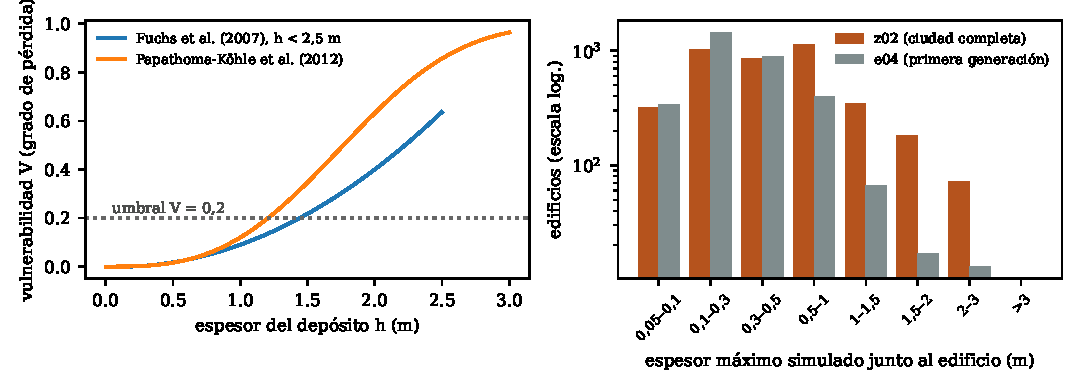
\includegraphics[width=\textwidth]{vulnerabilidad}
\caption{Izquierda: curvas de vulnerabilidad de \citet{fuchs2007} y \citet{papathoma2012} en función del espesor del depósito. Derecha: distribución del espesor máximo simulado junto a los edificios expuestos en el escenario seleccionado en la primera generación (escala logarítmica).}\label{fig:vulnerabilidad}
\end{figure}

\begin{table}[htbp]\centering\small
\caption{Pérdida relativa esperada con el espesor máximo simulado junto a cada edificio como intensidad. $\Sigma V$: pérdida relativa agregada (no es un conteo de edificios destruidos). Fuchs solo en su dominio ($h<\SI{2,5}{m}$); los edificios con $h\geq\SI{2,5}{m}$ se informan aparte. Viviendas: asignadas a los edificios con $V\geq0{,}2$.}\label{tab:danio}
\begin{adjustbox}{max width=\textwidth}\begin{tabular}{p{.34\textwidth}rrrrrrr}\toprule
Escenario & \multicolumn{3}{c}{Fuchs et al. (2007)} & \multicolumn{3}{c}{Papathoma-Köhle et al. (2012)} & $h\geq\SI{2,5}{m}$\\\cmidrule(lr){2-4}\cmidrule(lr){5-7}
 & $\Sigma V$ & Edif. $V\geq0{,}2$ & Viv. & $\Sigma V$ & Edif. $V\geq0{,}2$ & Viv. & Edif.\\\midrule
Seleccionada: cauce + brazos sur + lluvia (300 mil m³) & 187,1 & 271 & 366 & 275,8 & 425 & 593 & 15\\
Ídem con más rugosidad fuera de calles & 174,9 & 244 & 346 & 256,9 & 398 & 594 & 12\\
Solo cauce principal (300 mil m³) & 163,9 & 264 & 305 & 248,4 & 390 & 498 & 16\\
Solo cauce principal (150 mil m³) & 83,3 & 131 & 117 & 123,3 & 203 & 199 & 4\\
Hipotético: colector 30 m³/s & 121,3 & 169 & 151 & 181,2 & 264 & 246 & 12\\
Hipotético: colector 100 m³/s & 107,6 & 162 & 129 & 162,8 & 242 & 192 & 12\\
Primera generación (modelo con 1.103 edificios; exposición sobre 42.018 huellas) & 43,4 & 34 & 26 & 55,4 & 52 & 38 & 1\\
\bottomrule\end{tabular}\end{adjustbox}\end{table}

\paragraph{Daño esperado.} En el escenario seleccionado en la primera generación, la mayoría de los edificios expuestos tienen espesores menores a \SI{0,5}{m}, con una vulnerabilidad baja (figura~\ref{fig:vulnerabilidad}). La suma de pérdidas equivale a 44 edificios totalmente dañados con la curva de Fuchs y a 56 con la de Papathoma-Köhle. Entre 38 y 63 edificios tienen $V\geq0{,}2$, y entre 8 y 19, $V\geq0{,}5$. Las viviendas asignadas a los edificios con $V\geq0{,}2$ son 61 y 80, respectivamente (cuadro~\ref{tab:danio}).

\begin{figure}[htbp]\centering
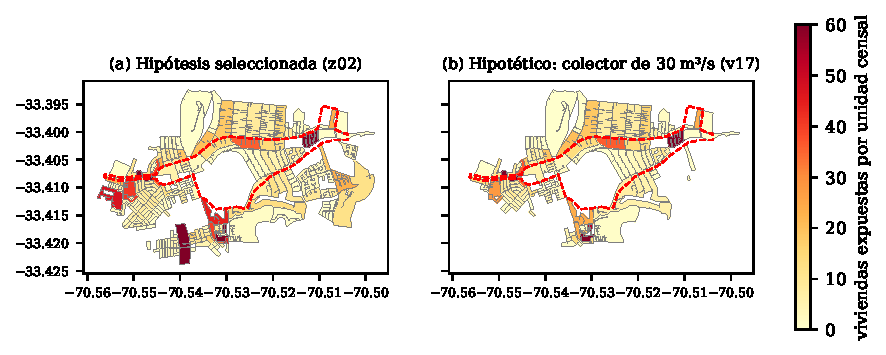
\includegraphics[width=\textwidth]{manzanas}
\caption{Viviendas expuestas por manzana (Censo 2017, ponderación areal) con más de \SI{5}{cm} de barro simulado. (a) Escenario seleccionado en la primera generación. (b) Escenario hipotético con capacidad del colector de Bulnes Correa fijada en 30 m$^3$/s).}\label{fig:manzanas}
\end{figure}

\paragraph{Contraste con las cifras oficiales.}
\begin{table}[htbp]\centering\small
\caption{Contraste con los balances oficiales preliminares del 9 de octubre de 2026 (escenario seleccionado en la primera generación).}\label{tab:contraste}
\begin{tabular}{p{.24\textwidth}p{.3\textwidth}p{.36\textwidth}}\toprule
Indicador & Cifra oficial & Este estudio\\\midrule
Viviendas afectadas & Senapred: 75 con daño mayor + 2.286 con daño menor = 2.361; municipio: 1.960--2.015 & 2.358 (A) y 2.947 (B) expuestas a más de \SI{5}{cm}; rango de sensibilidad: 2.061--3.235\\
Daño severo & Senapred: 75 con daño mayor; municipio: 55 inhabitables & 61--80 viviendas con $V\geq0{,}2$; 38--63 edificios con $V\geq0{,}2$; 44--56 edificios equivalentes de pérdida calculada\\
Calles dañadas & Municipio: \SI{15}{km} de avenidas & \SI{15,3}{km} de calles con barro, \SI{12,9}{km} de ellas avenidas\\
Personas & Senapred: 6 lesionados, 118 damnificados y 147 albergados (RM); unas 1.000 personas evacuadas & 7.844--9.713 personas residentes en el área con barro (concepto distinto: exposición)\\
\bottomrule\end{tabular}\end{table}
El cuadro~\ref{tab:contraste} resume el contraste. Descriptivamente, las viviendas expuestas del escenario seleccionado en la primera generación quedan en el mismo orden de magnitud que las viviendas afectadas informadas (HE1), y las viviendas con daño esperado significativo, en el orden de las de daño mayor (HE2); las categorías calculadas y administrativas no son equivalentes. Los escenarios con \SI{150000}{m^3} subestiman ambas cifras en un factor 2 a 3, lo que coincide con el estudio principal, que ya indicaba que el alcance observado favorece volúmenes mayores.

\section{Discusión}
\paragraph{Coherencia con lo observado.} Tres indicadores informados por las autoridades ---viviendas afectadas, daño severo y longitud de calles---, no utilizados para calibrar la propagación, quedan dentro de los rangos estimados para el escenario seleccionado en la primera generación. Es un contraste descriptivo: la comparación se realizó conociendo esos balances y no constituye validación independiente. Sin embargo, no es una validación ciega: los umbrales y los escenarios mostrados se eligieron conociendo los balances, y las cifras oficiales son preliminares.
\paragraph{Qué agrega la asignación dasimétrica.} El barro corre por calles bordeadas de casas, de modo que la población expuesta se concentra en los frentes de manzana. La ponderación areal reparte esa población por toda la manzana y puede estimar una exposición menor cuando el flujo solo toca un borde. La asignación por huella modifica esa distribución bajo sus propios supuestos, sin demostrar por sí sola una mayor exactitud; además supone que todas las huellas de 30 a \SI{2000}{m^2} son viviendas.
\paragraph{Límites de las curvas de vulnerabilidad.} Las curvas provienen de eventos alpinos con edificios de albañilería y hormigón. La tipología constructiva de las viviendas del área no se relevó en este estudio; a juzgar por las imágenes, predominan casas de uno o dos pisos con antejardín y cierre perimetral, que pueden retener parte del barro. Además, se usa el espesor máximo del flujo y no el del depósito, lo que tiende a sobrestimar el daño, y no se consideran la velocidad ni la presión dinámica. Por eso las cifras de daño deben leerse como un orden de magnitud.
\paragraph{Supuestos y sesgos.}
\begin{itemize}
\item El Censo 2017 no refleja el crecimiento posterior.
\item Las huellas detectadas automáticamente pueden fusionar o dividir edificios, y la asignación dasimétrica no distingue usos residenciales de no residenciales.
\item La propagación proviene de simulaciones de cribado sobre un terreno con pocas huellas de edificios; las simulaciones en curso con las 42.018 huellas pueden cambiar la extensión y las profundidades.
\item El daño a contenidos, a vehículos y a la infraestructura pública no se estima.
\end{itemize}

\section{Conclusiones}
\begin{enumerate}
\item En el escenario seleccionado en la primera generación, unas 2.400 a 2.900 viviendas y 7.800 a 9.700 personas se asignan, mediante los datos del Censo 2017, al área de alcance simulado por más de \SI{5}{cm} de barro. Es el mismo orden que las 2.361 viviendas afectadas del balance de Senapred.
\item El daño esperado, estimado con curvas de vulnerabilidad publicadas, se asigna a unas 60 a 80 viviendas que superan el umbral de pérdida esperada considerado. La comparación con las 75 viviendas con daño mayor y las 55 inhabitables informadas es descriptiva: las categorías no son equivalentes.
\item En este análisis, la asignación por huella de edificio representa de forma más localizada la exposición junto a las calles, bajo los supuestos adoptados.
\item El método es reproducible con datos públicos y puede adaptarse a otros eventos, explicitando el origen, la resolución y las limitaciones de la huella de propagación utilizada.
\item Las cifras son preliminares y se recalcularán con el modelo de propagación definitivo.
\end{enumerate}

\section*{Disponibilidad de datos y código}
{\sloppy Los programas \texttt{exposicion2.py} y \texttt{figura\_exposicion2.py}, y los resultados agregados (\texttt{res/exposicion2.json}), están en \url{https://aluvion.hirely.cl/datos.html}\allowbreak. Solo se publican agregados.}

\bibliographystyle{apacite}
\bibliography{referencias}
\end{document}
